%File: AnonymousSubmission2027.tex
\documentclass[letterpaper]{article} % DO NOT CHANGE THIS
\usepackage[submission]{aaai2027}  % DO NOT CHANGE THIS
% The serif, sans-serif, and monospaced fonts are loaded automatically by
% aaai2027.sty (newtxtext, helvet, courier). DO NOT add font packages.
\usepackage[hyphens]{url}  % DO NOT CHANGE THIS
\usepackage{graphicx} % DO NOT CHANGE THIS
\urlstyle{rm} % DO NOT CHANGE THIS
\def\UrlFont{\rm}  % DO NOT CHANGE THIS
\usepackage{natbib}  % DO NOT CHANGE THIS AND DO NOT ADD ANY OPTIONS TO IT
\usepackage{caption} % DO NOT CHANGE THIS AND DO NOT ADD ANY OPTIONS TO IT
\usepackage{amsmath}
\usepackage{amssymb}
\usepackage{multirow}
\usepackage{booktabs}
\newcommand{\thickhline}{\noalign{\hrule height 0.8pt}}
\frenchspacing  % DO NOT CHANGE THIS
\pdfinfo{
/TemplateVersion (2027.1)
}
\setcounter{secnumdepth}{2}

\title{MAReuse: Computation Reuse for Efficient Multi-Agent LLM Inference}
\author{Anonymous Submission}
\affiliations{}

\begin{document}

\maketitle

\begin{abstract}
Multi-agent large language model (LLM) systems improve complex problem solving by specializing roles, coordinating workflows, and integrating intermediate results. However, they incur substantial inference latency: prefill repeatedly recomputes KV caches for shared context, while decoding still generates similar token sequences autoregressively. Existing reuse techniques mainly reduce redundant prefill computation, leaving decoding-stage reuse across agents largely underexplored. We propose \textbf{MAReuse}, a computation reuse framework for multi-agent LLM inference that exploits structured redundancy across prefill and decoding. During prefill, MAReuse first repositions reused KV caches using RoPE, then selectively recomputes a small set of critical tokens to refine their KV states. We observe that first-layer token importance poorly predicts later-layer KV errors, so MAReuse re-selects these positions by their KV deviations at an intermediate filter layer. During decoding, MAReuse performs collaborative speculative decoding by hierarchically constructing linear drafts from exact history matches and falling back to a logits-cache tree when no valid match is available. The target model then verifies multiple draft tokens in one forward pass. We evaluate on three diverse public benchmarks. At comparable accuracy, MAReuse achieves the fastest prefill among the compared KV-cache reuse methods and the fastest decoding among the compared speculative decoding methods. Compared with standard multi-agent inference, MAReuse achieves up to 2.7$\times$ prefill speedup and 3.2$\times$ decoding speedup.
\end{abstract}

\section{Introduction}

Large language model agents are increasingly deployed as multi-agent systems. Different agents can assume specialized roles, exchange intermediate results, and aggregate predecessor outputs along a structured workflow \citep{li2023camel, zhang2025agentprune}. This paradigm improves the ability of LLMs to handle complex tasks, but it also creates new inference bottlenecks. Compared with a single-agent workflow, a multi-agent workflow repeatedly processes highly overlapping contexts, including task descriptions, shared evidence, and intermediate outputs generated by other agents, making multi-agent inference computationally expensive.

Existing work mainly reduces multi-agent prefill overhead by reusing KV caches from shared contexts. Prefix caching can reuse KV caches only when requests share an identical prompt prefix \citep{kwon2023vllm, zheng2024sglang}, and therefore cannot directly reuse shared content once its preceding prefix changes. Precomputed cache methods support reuse of non-prefix content \citep{yao2025cacheblend}, but may suffer accuracy degradation when applied to dynamic agent outputs. At the same time, there has been little focused study of how to exploit agent outputs from the same input instance and histories from previous input instances to accelerate the decoding stage with speculative decoding.

This paper proposes \textbf{MAReuse}, a computation reuse framework that accelerates both prefill and decoding for multi-agent LLM inference. During prefill, MAReuse reuses KV caches for content that can be aligned across agents and corrects the reused states by estimating token-wise KV deviations at an intermediate layer. The design is motivated by our observation that high-deviation tokens are not fully determined at the first layer: tokens with large KV deviations in shallow layers may not be the same tokens with large deviations in later layers. MAReuse therefore collects intermediate hidden states, re-selects a small set of high-deviation tokens at the filter layer, and recomputes only these positions to recover later-layer KV states with limited extra cost.

During decoding, MAReuse introduces collaborative speculative decoding. It does not rely on a draft model. Instead, it maintains a two-level retrieval memory. The local index records generated text from earlier agents within the same input instance, which we call in-sample cross-agent history. The global index organizes outputs from completed input instances grouped by agent role, which we call cross-sample role-aware history. MAReuse first constructs a linear draft from a valid exact match in the local or role-aware global index. If neither retrieval level returns such a match, it deterministically falls back to a tree-structured draft filled with candidate next tokens cached from verified logits, which we call a logits-cache tree draft. The target model then verifies the candidates and may accept multiple tokens in a single forward pass, increasing the number of accepted tokens per decoding step and improving generation throughput.

\begin{figure*}[t]
    \centering
    
\includegraphics[width=0.98\textwidth]{"Figures/Overview of MAReuse.pdf"}
    \caption{Overview of MAReuse. The framework reuses aligned KV caches during prefill with filter-layer correction and accelerates decoding with verifiable drafts from local outputs, role-aware history, and logits-cache trees.}
    \label{fig:mareuse-overview}
\end{figure*}

The contributions of this paper are:
\begin{itemize}
    \item We formulate multi-agent LLM inference as a cross-stage reuse problem, identifying reusable computation in repeated shared-context prefill and recurring generation patterns.
    \item We propose filter-layer corrected prefill reuse, which re-selects high-deviation tokens at an intermediate layer and recomputes only critical positions to improve reused KV states at low cost.
    \item We design collaborative speculative decoding that hierarchically retrieves linear continuations from local and role-aware histories and uses a logits-cache tree as a deterministic fallback. Across all evaluated datasets and workflow widths, MAReuse achieves average speedups of 2.00$\times$ in TTFT and 2.57$\times$ in decoding, with limited accuracy degradation in most settings.
\end{itemize}

\section{Related Work}

\subsection{LLM-Based Multi-Agent Collaboration}

LLM-based multi-agent systems commonly use role-based interaction as the basis of collaboration. Different agents are assigned specialized responsibilities or perspectives, which guide task decomposition, information exchange, debate, and result aggregation. Representative systems include CAMEL, ChatDev, and MAD \citep{li2023camel, qian2024chatdev, liang2024encouraging}. Later work further studies workflow orchestration and communication structure. AutoGen supports configurable message passing and dialogue control, while MetaGPT encodes structured multi-agent workflows through standard operating procedures \citep{wu2023autogen, hong2024metagpt}. GPTSwarm and AgentPrune further model and optimize information flow through graph structures \citep{zhuge2024gptswarm, zhang2025agentprune}.

\subsection{KV Cache Reuse}

KV cache reuse is an important direction for reducing LLM prefill cost. Prefix caching reuses previously computed KV caches when requests share an identical prompt prefix; vLLM and SGLang support efficient prefix sharing with PagedAttention and RadixAttention, respectively \citep{kwon2023vllm, zheng2024sglang}, and RAGCache extends this to retrieval-augmented generation \citep{jin2025ragcache}. These exact methods are limited by strict prefix matching. To reuse non-prefix content, TurboRAG stores KV caches for retrieved documents, while APE uses adaptive parallel encoding and lightweight calibration to approximate sequential prefill \citep{lu2025turborag, yang2025ape}. Selective correction methods further trade off efficiency and quality: CacheBlend selects tokens by first-layer KV deviations \citep{yao2025cacheblend}, EPIC heuristically recomputes the first few tokens of each block \citep{hu2025epic}, KVShare shares KV caches across requests with dual-stage high-deviation recomputation and cache-aware scheduling \citep{yang2025kvshare}, RelayCaching profiles layer ranges and sparse positions for multi-agent decode-to-prefill reuse \citep{geng2026relaycaching}, and KVCOMM estimates prefix-conditioned KV offsets with an online anchor pool \citep{ye2025kvcomm}. Query-aware token selection methods such as $A^3$ and ProphetKV are mainly designed for RAG scenarios, where the user query is usually placed at the end of the prompt \citep{zhou2025a3, wang2026prophetkv}; this differs from our interleaved multi-agent prompts.

\subsection{Speculative Decoding}

Speculative decoding reduces serial autoregressive steps by generating draft tokens and verifying them in parallel with the target model. Training-free methods retrieve candidates from repeated prompt fragments, as in Prompt Lookup Decoding \citep{saxena2023promptlookup}, or improve candidate construction with logits and automaton indices: Token Recycling builds logits trees from top-$k$ candidates, SAM-Decoding retrieves suffix-automaton matches, and RACER combines logits trees with Aho-Corasick retrieval \citep{luo2025tokenrecycling, hu2025sam, zhang2026racer}. These methods improve draft coverage but mostly target single-request or single-agent contexts. Model-based methods such as EAGLE-3 and DSpark train dedicated draft components \citep{li2025eagle3, cheng2026dspark}; in contrast, MAReuse requires no additional model training and constructs drafts from in-sample cross-agent outputs and cross-sample role-aware history.


\section{Observations}

We model multi-agent inference as a directed acyclic graph $G=(V,E)$ of LLM calls. Each node $v\in V$ corresponds to one agent invocation, and each edge transfers generated text from a predecessor agent to a successor prompt. The prompt of node $v$ can be written as an alternating sequence of static template segments and dynamic placeholders:
\begin{equation}
P_v = [a_0, z_1, a_1, \ldots, z_m, a_m],
\label{eq:prompt-decomposition}
\end{equation}
where $[\cdot]$ denotes concatenation of prompt segments, $a_i$ denotes fixed role instructions, few-shot examples, or template text, and $z_i$ denotes dynamic content such as the user question, predecessor output, or auxiliary condition text. Since node outputs are inserted into successor prompts, text that has already been computed within a single workflow execution is repeatedly encoded by downstream nodes. If a workflow contains $M$ sequentially related calls and each step adds an average context length $L$, the accumulated prefill token-processing volume is approximately $O(\sum_i iL)=O(M^2L)$, before accounting for the sequence-length-dependent cost of attention. Meanwhile, the agents perform $O(MY)$ autoregressive token-generation steps when each agent generates an average of $Y$ tokens. Although this number is linear in output length, decoding remains a major latency bottleneck because token generation is inherently sequential.

\subsection{(Observation 1) Layer-1 Value Deviation Misses Later-Layer Errors}

As discussed above, directly reusing another agent's output KV cache can cause substantial KV mismatch, since the receiving agent conditions the same output on a different prefix. Selectively recomputing a few influential tokens can reduce deviations from full-prefill KV states and better recover cross-block attention. A representative token selection method is CacheBlend \citep{yao2025cacheblend}, which ranks reused tokens by K or V deviation. For a comparison layer $\ell$ (with layers indexed from 0), let $\tilde V_i^\ell$ denote the value state from pure cache concatenation with RoPE alignment~\citep{su2021roformer}, and let $V_i^\ell$ denote the exact value state under the current full prompt. We use value deviation to define the selected set:
\begin{equation}
\mathcal S_\ell =
\operatorname{Top}_{\rho}
\{\|V_i^\ell-\tilde V_i^\ell\|_2^2\}_i .
\end{equation}
Here $\operatorname{Top}_{\rho}$ returns the top-$\rho$ fraction of reused-token indices. The same definition can be applied with key deviation. CacheBlend selects $\mathcal S_1$, i.e., the tokens with the largest layer-1 deviation, and uses this fixed set for recomputation in all later layers. We conduct this analysis on HotpotQA~\citep{yang2018hotpotqa}, a multi-hop RAG dataset. We compare $\mathcal S_1$, $\mathcal S_6$, and $\mathcal S_{16}$ with $\mathcal S_f$ at a later layer $f$. We set $\rho=20\%$ and report their Jaccard similarities with $\mathcal S_f$. If layer-1 deviations were stable proxies for later, their overlap with middle and deep layers would remain high.

\begin{table}[t]
\centering
\setlength{\tabcolsep}{4.7pt}
\begin{tabular}{lcccc}
\hline
\addlinespace[1pt]
Comparison layer $f$ & 4 & 6 & 16 & 24 \\
\hline
\addlinespace[1pt]
$\operatorname{Jaccard}(\mathcal S_1,\mathcal S_f)$ & 0.7425 & 0.5736 & 0.6333 & 0.4926 \\
$\operatorname{Jaccard}(\mathcal S_6,\mathcal S_f)$ & 0.8397 & 1.0000 & 0.7569 & 0.6947 \\
$\operatorname{Jaccard}(\mathcal S_{16},\mathcal S_f)$ & 0.6944 & 0.7569 & 1.0000 & 0.8971 \\
\addlinespace[1pt]
\hline
\end{tabular}
\caption{Layer-wise drift of high-deviation token selection.}
\label{tab:layer-drift}
\end{table}

Table~\ref{tab:layer-drift} shows that layer-1 selection drifts substantially from middle and deep layers, with its Jaccard similarity dropping to 0.4926 at layer 24. In contrast, selections from later layers better match nearby and deeper layers, with $\mathcal S_{16}$ maintaining a 0.8971 overlap with layer 24. Thus, relying only on the initial high-deviation token selection may be unreliable for later-layer errors.

\subsection{(Observation 2) Multi-Agent Outputs Contain Long Exact Reuse Spans}

To conservatively estimate reuse opportunities during decoding, let $Y=(y_1,\ldots,y_n)$ be an agent output sequence and let $S$ be a candidate source sequence, such as prior agent outputs, few-shot examples, or the user question. For each output position $i$, $L_i$ denotes the longest exact contiguous span starting at $i$ that also appears in $S$:
\begin{equation}
L_i=\max\{\ell \mid \exists j,\;Y_{i:i+\ell-1}=S_{j:j+\ell-1}\}.
\end{equation}
Here $j$ indexes the matching start position in $S$, and $\ell$ is the length of the exact match.
The coverage by spans of length at least $k$ is
\begin{equation}
\begin{gathered}
\mathrm{Coverage}_{\ge k}(Y,S)
=\frac{1}{n}\left|\bigcup_{i:L_i\ge k} A_i\right|,\\
\text{where } A_i=[i,i+L_i-1]\cap[1,n].
\end{gathered}
\end{equation}
This metric measures how much of the output is covered by long exact spans from the candidate source.

\begin{table}[t]
\centering
\begin{tabular}{lcccc}
\hline
\addlinespace[1pt]
Scenario & $\ge4$ & $\ge8$ & $\ge16$ & Avg. longest \\
\hline
\addlinespace[1pt]
Spec-Bench & 25.0\% & 13.0\% & 5.2\% & 13.6 \\
\addlinespace[1pt]
Multi-Agent & 47.0\% & 26.0\% & 17.8\% & 38.8 \\
\addlinespace[1pt]
\hline
\end{tabular}
\caption{Exact-span reuse coverage and longest matches in ordinary and multi-agent outputs.}
\label{tab:coverage}
\end{table}

Table~\ref{tab:coverage} shows that multi-agent decoding is far from purely novel token generation. Compared with ordinary Spec-Bench samples~\citep{xia2024unlocking}, multi-agent outputs on GSM8K~\citep{cobbe2021training} contain much stronger long-span reuse: $\mathrm{Coverage}_{\ge16}$ rises from 5.2\% to 17.8\%, and the average longest match increases from 13.6 to 38.8 tokens. We further observe that reuse opportunities increase with workflow width: $\mathrm{Coverage}_{\ge16}$ is 12.0\%, 18.2\%, and 21.1\% for workflows with 3, 4, and 5 agents, respectively.

\subsection{(Observation 3) Same-Role Histories Contain Cross-Sample Reuse}

In-sample history is limited to text generated within the current sample. We therefore examine whether outputs from the same agent role contain reusable continuations across samples.

\begin{table}[t]
\centering
%\small
\setlength{\tabcolsep}{3pt}
\begin{tabular}{lcc}
\hline
\addlinespace[1pt]
History source & Cov. $\ge8$ & Avg. longest \\
\hline
\addlinespace[1pt]
In-sample history & 26.0\% & 38.8 \\
\addlinespace[1pt]
Cross-sample same-role history & 10.4\% & 24.1 \\
\addlinespace[1pt]
Cross-sample diff-role history & 2.8\% & 11.7 \\
\addlinespace[1pt]
\hline
\end{tabular}
\caption{Reuse potential of different history sources.}
\label{tab:cross-sample-reuse}
\end{table}

Table~\ref{tab:cross-sample-reuse} compares different history sources using the metrics defined above. In-sample history remains the strongest source, with 26.0\% coverage and an average longest match of 38.8 tokens. Cross-sample same-role history reaches 10.4\% coverage and 24.1 tokens, substantially outperforming different-role history at 2.8\% and 11.7 tokens. This result supports role-aware global history as a complementary source when local reuse is unavailable.

\section{MAReuse}

\subsection{Overview}

Figure~\ref{fig:mareuse-overview} illustrates the overall workflow of MAReuse. Given a fixed multi-agent workflow, MAReuse accelerates inference without adding a draft model or changing the generation policy. As agents execute, they produce token sequences along with reusable byproducts of target-model computation, including KV caches, auxiliary hidden states, and logits from verified decoding steps. Token ids provide the sequence anchors for both prompt reconstruction and history matching; KV caches, together with hidden states, help avoid redundant prefill computation; and cached logits provide alternative next-token candidates for constructing fallback tree drafts. 

\subsection{Prefill Reuse with Filter-Layer Correction}

Following the prompt decomposition in Eq.~\eqref{eq:prompt-decomposition}, MAReuse precomputes the KV cache for each static segment $a_i$ during graph initialization and writes it into shared KV memory. During sample execution, the KV caches of the user question, agent responses, and generated conditions are also written into the same memory for use by successor nodes.

To build the reused prompt for node $v$, MAReuse fetches the token ids and KV cache of each segment from shared memory and concatenates them according to Eq.~\eqref{eq:prompt-decomposition}. Because RoPE ties keys and queries to token positions~\citep{su2021roformer}, MAReuse realigns each cached chunk to its starting position in the assembled prompt, avoiding the positional mismatch known to affect non-prefix KV reuse~\citep{liu2026cacheslide}.

Directly concatenating cached chunks is inaccurate because the chunks are placed under a different prefix and context. A common remedy is to select a small fraction of tokens and recompute their KV states under the current prompt. However, as shown in \textbf{Observation 1}, selecting this correction set only from layer-1 deviations, as in CacheBlend, can miss tokens that become important in intermediate layers.

MAReuse addresses this issue with filter-layer correction. We use $f$ to denote the transformer block at which full-sequence filtering is performed. The filter layer $f$ is selected offline by evaluating candidate layers on the target model, as illustrated in Figure~\ref{fig:filter-layer-sweep}, and then fixed during inference. For a candidate filter layer, we measure how much correction reduces the deviation:
\begin{equation}
\begin{aligned}
G_\ell&=\frac{1}{n}\sum_{i=1}^{n}\|V_i^\ell-\hat V_i^\ell\|_2^2,\\
\mathrm{Reduction}
&=\frac{\sum_{\ell\in\mathcal L}(G_\ell-G_\ell')}{\sum_{\ell\in\mathcal L}G_\ell}.
\end{aligned}
\end{equation}
where $G_\ell$ and $G_\ell'$ are the layer-$\ell$ deviations before and after correction, respectively. In Figure~\ref{fig:filter-layer-sweep}, we set $\mathcal L$ to all transformer layers and report the overall reduction.

With the offline-selected filter layer $f$, when a reusable chunk is first produced, MAReuse records the hidden states at the input of block $f$, together with its token ids and KV cache. These stored states avoid full-sequence recomputation through the blocks preceding $f$. When assembling a prompt from reusable chunks, MAReuse first applies RoPE-only alignment to their cached states. It then selects high-deviation tokens at layer 1 and propagates only these positions through the remaining blocks before $f$ as an initial correction. At block $f$, MAReuse merges the recomputed hidden states of these positions with the stored hidden states of the remaining positions and runs one full-sequence block computation to obtain the filter-layer KV states. Comparing these states with the aligned reused KV states lets MAReuse re-select the largest-deviation tokens. Only the re-selected positions are recomputed to correct the reused KV cache, while the remaining positions continue to use the aligned reused states.

\begin{figure}[t]
\centering
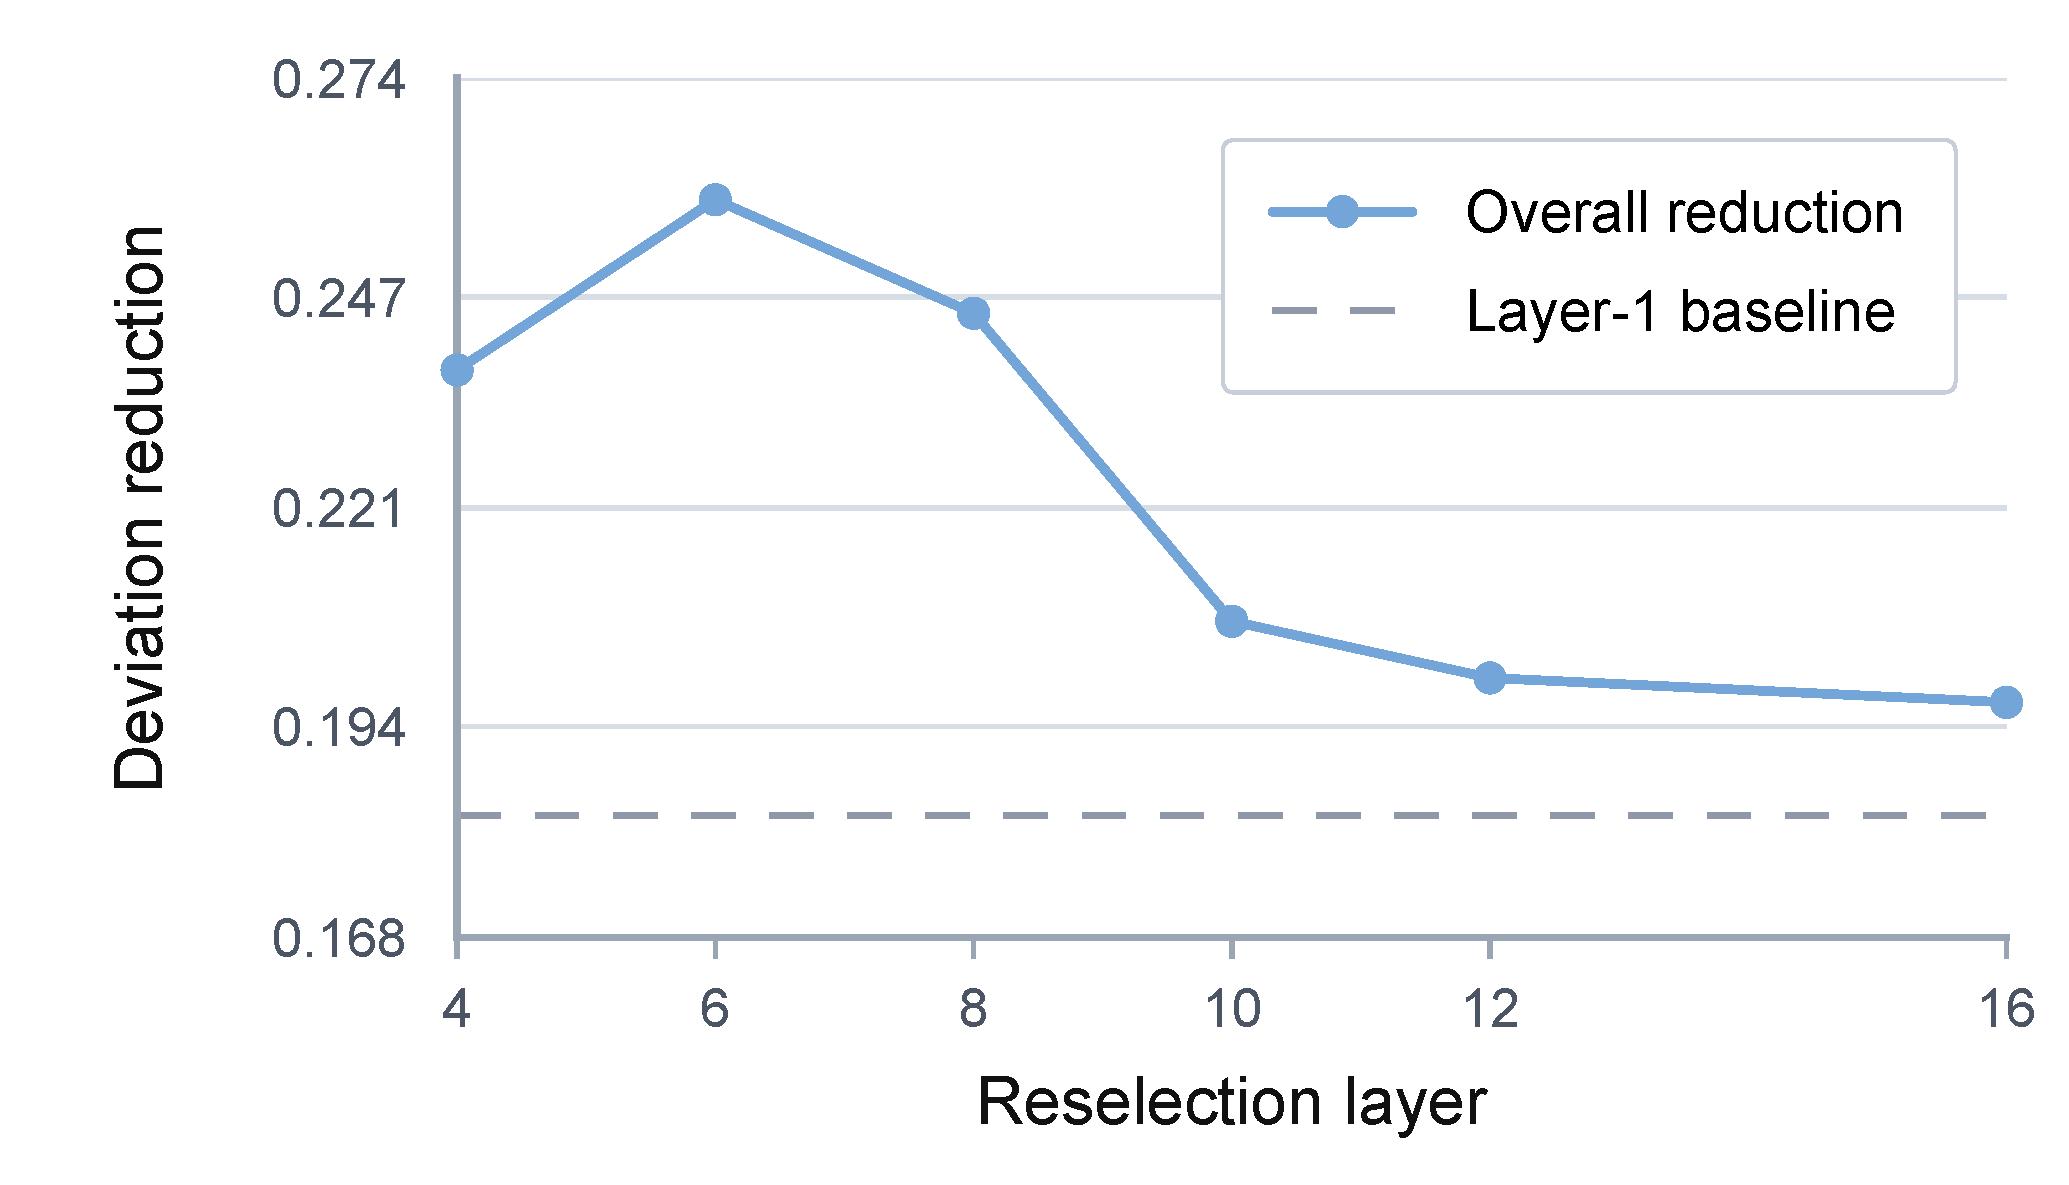
\includegraphics[width=\columnwidth]{Figures/layer_sweep_v.pdf}
\caption{Offline layer sweep for selecting the filter layer, evaluated on Llama-3.1-8B with GSM8K.}
\label{fig:filter-layer-sweep}
\end{figure}

\subsection{Collaborative Speculative Decoding}

\subsubsection{Local Retrieval with a Dynamic Suffix Automaton}

MAReuse constructs speculative drafts from multi-agent generation histories whose tokens have already been generated or verified by the target model. \textbf{Observation 2} shows that multi-agent outputs contain many long exact reuse spans, especially reusable intermediate content generated by other agents earlier within the same sample. To capture these local reuse opportunities, MAReuse uses a dynamic suffix automaton (SAM) as the local index.

A suffix automaton compactly represents all substrings of the inserted token history and supports online fallback through suffix links to find the longest available match. The SAM is initialized empty at the start of each sample and released after the sample finishes, restricting the local index to current-sample histories. At each speculative decoding step, MAReuse queries the SAM for the longest in-sample suffix match and uses the following tokens as a linear draft; after verification, the accepted tokens are inserted back into the SAM. This dynamic-anchor design avoids committing to a fixed anchor length: short fixed anchors are easy to match but weakly constrained, while long fixed anchors impose strict matching requirements and may miss reuse opportunities. As shown in Table~\ref{tab:local-sam-ablation}, dynamic matching outperforms fixed $n$-gram anchors in throughput and mean accepted tokens.

\begin{table}[!t]
\centering
\setlength{\tabcolsep}{8pt}
\begin{tabular}{lcc}
\hline
Local retriever & Mean tok/s & Mean accepted \\
\hline
Local SAM & 130.69 & 4.38 \\
Fixed 3-gram & 122.80 & 4.11 \\
Fixed 5-gram & 125.66 & 4.24 \\
Fixed 8-gram & 124.47 & 4.21 \\
Fixed 16-gram & 117.42 & 3.89 \\
\hline
\end{tabular}
\caption{Local retriever ablation on GSM8K. Local SAM outperforms fixed local $n$-gram anchors.}
\label{tab:local-sam-ablation}
\end{table}

\subsubsection{Role-Aware Global Retrieval}

Motivated by Observation 3, MAReuse queries a role-aware global index after a local miss. The global index is organized by role, anchor length, and exact anchor tokens; each matched key points to a bounded set of source-span references rather than duplicated continuation tokens. Outputs from completed samples are enumerated with three fixed anchor lengths and committed to the corresponding role-specific partition. During lookup, MAReuse tries longer anchors first and selects a referenced continuation using lightweight evidence such as historical hits, recency, and available continuation length. The index can optionally prune cold anchors for memory control, while the main experiments keep the unpruned index to isolate the effect of cross-sample reuse.

\subsubsection{Logits-Cache Tree Fallback}

When neither retrieval level returns a valid exact match, MAReuse deterministically falls back to a logits-cache tree draft, as illustrated in Figure~\ref{fig:tree-draft}. A local match is valid when its exact matched suffix reaches the configured minimum length, while a global match is obtained through one of the configured role-specific exact anchors. The cache maps each verified token id to its top-$k$ next-token ids. Starting from the current token, the module fills a fixed tree template by looking up the token at each node and placing its cached successors at adjacent child nodes. For each verification forward, MAReuse derives the required tree attention mask and position ids from this adjacency and uses leaf retrieval indices to recover candidate paths after target-model verification. Posterior verification then selects the accepted path. For a linear draft, the same verification procedure reduces to parallel checking along a single sequence.

The tree size controls how many candidate branches can be covered by one verification step. Larger trees may increase the mean number of accepted tokens per step (MAT), but they also increase the cost of each verification forward. MAReuse starts with a large tree template and specializes it online by recording target-model-verified selected paths from early evaluated samples and greedily retaining nodes that cover frequent historical paths, yielding a smaller frozen template for subsequent samples.

\begin{figure}[t]
    \centering
    
\includegraphics[width=\columnwidth]{"Figures/tree draft.pdf"}
    \caption{Logits-cache tree drafting and template specialization. Cached logits fill an initial fixed tree template, which is pruned using target-model-verified selected paths from early evaluated samples.}
    \label{fig:tree-draft}
\end{figure}


\begin{figure*}[t]
\centering
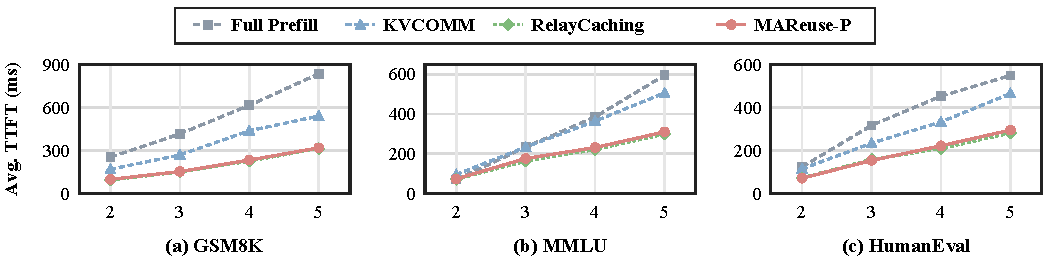
\includegraphics[width=\textwidth]{Figures/mareuse_p_total_ttft_tight.pdf}
\caption{Average per-sample TTFT comparison of Full Prefill, KVCOMM, RelayCaching, and MAReuse-P. The x-axis denotes workflow width, i.e., the number of agents. Lower values indicate better performance.}
\label{fig:prefill-ttft}
\end{figure*}

\section{Experiments}

\subsection{Experimental Setup}

\textbf{Datasets and Models.}
Following KVCOMM~\citep{ye2025kvcomm}, we evaluate MAReuse on multi-agent systems across three benchmarks: GSM8K~\citep{cobbe2021training} for mathematical reasoning, MMLU~\citep{hendrycks2021measuring} for knowledge question answering, and HumanEval~\citep{chen2021evaluating} for code generation. GSM8K and MMLU use Llama-3.1-8B-Instruct, while HumanEval uses Qwen2.5-Coder-7B-Instruct. Experiments are implemented with PyTorch 2.11.0 and Transformers 4.50.2 and conducted on an NVIDIA GeForce RTX 4090 GPU. Unless otherwise stated, all methods use the same multi-agent workflow and greedy decoding.

\noindent\textbf{Baselines.}
For prefill, Full Prefill denotes standard prefill without KV reuse, while MAReuse-P denotes MAReuse with only prefill reuse. We compare MAReuse-P with CacheBlend~\citep{yao2025cacheblend}, EPIC~\citep{hu2025epic}, RelayCaching~\citep{geng2026relaycaching}, and KVCOMM~\citep{ye2025kvcomm}. For decoding, Autoregressive denotes standard target-model decoding without speculation, and MAReuse-D denotes MAReuse with only collaborative speculative decoding enabled. We compare MAReuse-D with retrieval-based speculative decoding methods that do not require an auxiliary draft model: Token Recycling~\citep{luo2025tokenrecycling}, RACER~\citep{zhang2026racer}, and SAM-Decoding~\citep{hu2025sam}.

\noindent\textbf{Evaluation Metrics.}
For prefill reuse, we report task accuracy and time to first token (TTFT), where lower TTFT is better. For collaborative speculative decoding, we report generation throughput and MAT.

Detailed hyperparameters for MAReuse and all baselines, including recomputation ratios, filter-layer choices, retrieval anchors, draft budgets, and tree configurations, are provided in the supplementary material.

\subsection{Main Results}

\subsubsection{Prefill Results}

\begin{table}[t]
\centering
\small
\setlength{\tabcolsep}{5.2pt}
\begin{tabular}{clrrrr}
\thickhline
\textbf{Dataset} & \textbf{Method} & \textbf{2A} & \textbf{3A} & \textbf{4A} & \textbf{5A} \\
\hline
\addlinespace[1pt]
\multicolumn{6}{l}{\textbf{\textit{Llama-3.1-8B-Instruct (Accuracy \%)}}} \\
\addlinespace[1pt]
\hline
\addlinespace[1pt]
\multirow{6}{*}{GSM8K} & Full Prefill & 84.67 & 84.37 & 84.37 & 84.07 \\
\cline{2-6}
\addlinespace[1pt]
 & CacheBlend & 81.34 & 78.15 & 79.36 & 79.36 \\
 \addlinespace[1pt]
 & EPIC & 79.67 & 76.93 & 75.42 & 78.45 \\
 \addlinespace[1pt]
 & RelayCaching & 82.40 & 82.55 & 81.18 & 78.76 \\
 \addlinespace[1pt]
 & KVCOMM & \underline{83.46} & \textbf{83.16} & \underline{82.85} & \underline{82.25} \\
 \addlinespace[1pt]
 & MAReuse-P & \textbf{83.76} & \underline{82.70} & \textbf{83.01} & \textbf{82.40} \\
\hline
\addlinespace[1pt]
\multirow{6}{*}{MMLU} & Full Prefill & 64.71 & 84.31 & 80.39 & 82.35 \\
\cline{2-6}
\addlinespace[1pt]
 & CacheBlend & \underline{79.08} & \textbf{80.39} & 67.97 & 65.35 \\
 \addlinespace[1pt]
 & EPIC & 66.66 & \underline{79.73} & 58.82 & 58.82 \\
 \addlinespace[1pt]
 & RelayCaching & 76.47 & 73.86 & \underline{69.28} & 67.32 \\
 \addlinespace[1pt]
 & KVCOMM & 64.71 & 78.43 & \textbf{79.08} & \textbf{80.39} \\
 \addlinespace[1pt]
 & MAReuse-P & \textbf{81.70} & \textbf{80.39} & \textbf{79.08} & \underline{79.08} \\
\thickhline
\addlinespace[1pt]
\multicolumn{6}{l}{\textbf{\textit{Qwen2.5-Coder-7B-Instruct (Pass@1 \%)}}} \\
\addlinespace[1pt]
\hline
\addlinespace[1pt]
\multirow{6}{*}{HumanEval} & Full Prefill & 86.96 & 85.71 & 85.71 & 85.71 \\
\cline{2-6}
\addlinespace[1pt]
 & CacheBlend & 85.71 & 83.85 & \underline{86.34} & 84.47 \\
 \addlinespace[1pt]
 & EPIC & \underline{86.96} & \underline{86.34} & 86.96 & \underline{85.09} \\
 \addlinespace[1pt]
 & RelayCaching & 85.09 & 83.23 & 83.23 & 83.85 \\
 \addlinespace[1pt]
 & KVCOMM & \underline{86.96} & \underline{86.34} & \textbf{86.96} & \textbf{86.34} \\
 \addlinespace[1pt]
 & MAReuse-P & \textbf{87.58} & \textbf{87.58} & \underline{86.34} & \textbf{86.34} \\
\thickhline
\end{tabular}
\caption{Columns indicate the number of agents in the workflow, where A denotes agents. Bold indicates the best performance among reuse methods, and underline marks the second best.}
\label{tab:prefill-results}
\end{table}

Table~\ref{tab:prefill-results} and Figure~\ref{fig:prefill-ttft} jointly show the quality-latency tradeoff of prefill reuse. MAReuse-P largely preserves task accuracy with only modest drops from dense prefilling. The lower MMLU accuracy in the 2-agent setting is also noted by KVCOMM, where the first agent supplies keywords and the final agent sometimes answers without sufficient analysis. Among the baselines, KVCOMM achieves strong accuracy, but still suffers from high TTFT because unmatched segments fall back to dense prefill, while anchor-pool matching and offset estimation introduce additional overhead. MAReuse-P reduces average per-sample TTFT by 43.6\% on average compared with KVCOMM. CacheBlend and EPIC have TTFT close to MAReuse-P and are omitted from Figure~\ref{fig:prefill-ttft} for readability. RelayCaching is also close to MAReuse-P in TTFT, suggesting that skipping correction for a few layers brings only marginal latency savings in our setting. In contrast, MAReuse-P improves accuracy over RelayCaching by 4.7 points on average.

\subsubsection{Decoding Results}

\begin{table*}[t]
\centering
\small
\setlength{\tabcolsep}{11pt}
\begin{tabular}{clrrrrrrrr}
\thickhline
\textbf{Dataset} & \textbf{Method} & \multicolumn{4}{c}{\textbf{Throughput (tokens/s)}} & \multicolumn{4}{c}{\textbf{MAT}} \\
\cline{3-6}\cline{7-10}
 & & \textbf{2A} & \textbf{3A} & \textbf{4A} & \textbf{5A} & \textbf{2A} & \textbf{3A} & \textbf{4A} & \textbf{5A} \\
\hline
\addlinespace[1pt]
\multirow{5}{*}{GSM8K} & Autoregressive & 45.11 & 45.53 & 45.06 & 45.24 & 1.000 & 1.000 & 1.000 & 1.000 \\
 \addlinespace[1pt]
 & Token Recycling & 89.77 & 98.41 & 100.49 & 98.58 & 2.907 & 3.212 & 3.247 & 3.295 \\
 \addlinespace[1pt]
 & RACER & \underline{90.24} & 113.25 & 112.37 & 118.46 & \underline{2.964} & \underline{3.624} & 3.656 & 3.889 \\
 \addlinespace[1pt]
 & SAM-Decoding & 88.24 & \underline{114.06} & \underline{114.25} & \underline{124.59} & 2.786 & 3.600 & \underline{3.692} & \underline{4.040} \\
 \addlinespace[1pt]
 & MAReuse-D & \textbf{95.61} & \textbf{121.73} & \textbf{124.01} & \textbf{130.69} & \textbf{3.082} & \textbf{3.952} & \textbf{4.077} & \textbf{4.384} \\
\hline
\addlinespace[1pt]
\multirow{5}{*}{MMLU} & Autoregressive & 48.01 & 47.59 & 47.28 & 46.97 & 1.000 & 1.000 & 1.000 & 1.000 \\
 \addlinespace[1pt]
 & Token Recycling & 84.44 & 90.44 & 92.86 & 94.28 & 2.685 & 2.793 & 2.767 & 2.821 \\
 \addlinespace[1pt]
 & RACER & 84.62 & \underline{94.41} & \textbf{95.08} & \textbf{102.09} & 2.654 & \underline{2.905} & \textbf{2.867} & \underline{3.081} \\
 \addlinespace[1pt]
 & SAM-Decoding & \underline{87.72} & 90.03 & 91.18 & \underline{101.41} & \underline{2.687} & 2.823 & 2.733 & 2.984 \\
 \addlinespace[1pt]
 & MAReuse-D & \textbf{90.97} & \textbf{96.54} & \underline{94.87} & 101.39 & \textbf{2.713} & \textbf{2.938} & \underline{2.845} & \textbf{3.089} \\
\hline
\addlinespace[1pt]
\multirow{5}{*}{HumanEval} & Autoregressive & 51.49 & 51.78 & 51.20 & 52.17 & 1.000 & 1.000 & 1.000 & 1.000 \\
 \addlinespace[1pt]
 & Token Recycling & 117.60 & 114.34 & 112.31 & 107.14 & 2.998 & 3.127 & 3.173 & 3.059 \\
 \addlinespace[1pt]
 & RACER & 143.73 & \underline{127.80} & 132.89 & 124.06 & 3.939 & \underline{3.644} & 3.904 & 3.682 \\
 \addlinespace[1pt]
 & SAM-Decoding & \underline{161.16} & 127.29 & \underline{137.21} & \underline{126.54} & \underline{4.463} & 3.622 & \underline{4.108} & \underline{3.764} \\
 \addlinespace[1pt]
 & MAReuse-D & \textbf{166.01} & \textbf{131.18} & \textbf{141.13} & \textbf{132.28} & \textbf{4.774} & \textbf{3.818} & \textbf{4.254} & \textbf{4.009} \\
\thickhline
\end{tabular}
\caption{Collaborative speculative decoding improves generation throughput. Columns indicate workflow width, where A denotes agents. Bold marks the best value, and underline marks the second best.}
\label{tab:decoding-results}
\end{table*}

Table~\ref{tab:decoding-results} shows that MAReuse-D achieves the highest throughput in all settings on GSM8K and HumanEval. The gain comes from reusable continuations in multi-agent collaboration: later agents often build on earlier agents' outputs, allowing MAReuse-D to accept more tokens per verification step. The local index, role-aware global index, and logits-cache tree complement each other to provide robust draft construction across different reuse opportunities. On MMLU, the gains are smaller because this question-answering benchmark offers fewer long, contiguous, linear drafts; nevertheless, MAReuse-D remains competitive with the strongest prior and faster than autoregressive decoding.

\subsubsection{Combined Results}

\begin{table}[t]
\centering
\small
\setlength{\tabcolsep}{3.6pt}
\begin{tabular}{llcccc}
\thickhline
\textbf{Dataset} & \textbf{Agents} & \textbf{Base Acc.} & \textbf{Acc.} & \textbf{TTFT Sp.} & \textbf{Dec. Sp.} \\
\hline
\multirow{4}{*}{GSM8K} & 2A & 84.67 & 83.16 & 2.66$\times$ & 2.12$\times$ \\
 & 3A & 84.37 & 82.55 & 2.72$\times$ & 2.65$\times$ \\
 & 4A & 84.37 & 83.16 & 2.62$\times$ & 2.71$\times$ \\
 & 5A & 84.07 & 83.46 & 2.62$\times$ & 2.87$\times$ \\
\hline
\multirow{4}{*}{MMLU} & 2A & 64.71 & 81.05 & 0.95$\times$ & 2.01$\times$ \\
 & 3A & 84.31 & 80.39 & 1.33$\times$ & 2.01$\times$ \\
 & 4A & 80.39 & 77.37 & 1.67$\times$ & 2.12$\times$ \\
 & 5A & 82.35 & 76.47 & 1.92$\times$ & 2.29$\times$ \\
\hline
\multirow{4}{*}{HumanEval} & 2A & 86.96 & 86.34 & 1.71$\times$ & 3.01$\times$ \\
 & 3A & 85.71 & 85.09 & 1.89$\times$ & 3.21$\times$ \\
 & 4A & 85.71 & 85.09 & 2.06$\times$ & 3.05$\times$ \\
 & 5A & 85.71 & 84.47 & 1.86$\times$ & 2.81$\times$ \\
\thickhline
\end{tabular}
\caption{Combined acceleration with both prefill reuse and collaborative decoding enabled. Speedups are measured against the unoptimized multi-agent baseline without KV-cache reuse or speculative decoding.}
\label{tab:combined-results}
\end{table}

Table~\ref{tab:combined-results} compares the full MAReuse pipeline with the original multi-agent pipeline using full prefill and autoregressive decoding. Since MAReuse-P reduces TTFT and MAReuse-D reduces decoding latency, the combined system improves both metrics in most settings, with particularly strong gains on larger-agent GSM8K and HumanEval workflows. Accuracy drops on MMLU are slightly larger than those on GSM8K and HumanEval. The 0.95$\times$ TTFT speedup in the 2-agent setting arises because the prompts contain too few tokens to amortize the overhead of KV cache reuse, making full prefill slightly faster.

\subsection{Ablation Study}

\subsubsection{Filter-Layer Selection}

Figure~\ref{fig:ablation-filter-layer} evaluates filter-layer placement in MAReuse-P under the same correction budget. We observe two trends. First, the accuracy curve is consistent with the offline sweep in Figure~\ref{fig:filter-layer-sweep}: intermediate layers, especially layer 6, give stronger average accuracy than very shallow or very deep layers. Second, accuracy drops faster at deeper layers as the number of agents increases, indicating that wider workflows are more sensitive to late correction.

\begin{figure}[t]
\centering
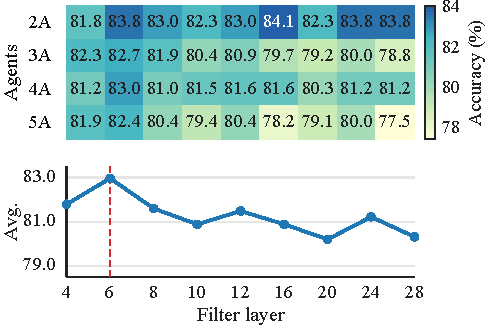
\includegraphics[width=0.98\columnwidth]{Figures/ablation_filter_layer_tight.pdf}
\caption{Effect of filter-layer selection on GSM8K accuracy. The heatmap reports accuracy across workflow widths; the lower curve reports the average.}
\label{fig:ablation-filter-layer}
\end{figure}

\begin{figure}[!ht]
\centering
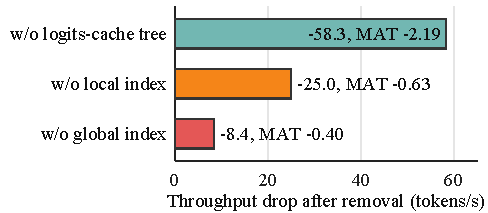
\includegraphics[width=0.98\columnwidth]{Figures/ablation_components_tight.pdf}
\caption{Leave-one-out ablation of MAReuse-D components on GSM8K 5A. Bars show the throughput and MAT drops after removing each component.}
\label{fig:ablation-components}
\end{figure}

\subsubsection{Decoding Components}
Figure~\ref{fig:ablation-components} shows that the logits-cache tree is the foundation of MAReuse-D: removing it causes the largest drop, from 130.69 to 72.42 tokens/s and from 4.384 to 2.19 MAT, because it preserves draft coverage when retrieval is weak. The local and role-aware global indices are also indispensable: removing them lowers throughput to 105.71 and 122.33 tokens/s, respectively. These results show that local cross-agent reuse and global role-aware reuse complement each other, jointly forming an integrated draft mechanism with the logits-cache tree.

\section{Conclusion}

Overall, the results show that multi-agent inference contains exploitable redundancy beyond repeated prompt prefixes. By correcting reused KV states during prefill and turning agent histories into verifiable drafts during decoding, MAReuse converts both shared context and recurring generation patterns into practical acceleration opportunities. Across tasks, these gains indicate that reuse can accelerate the inference pipeline while preserving quality in most settings.

\bibliography{aaai2027}

\end{document}
